\chapter{Umsetzung} %Should be roughly 18pages
\label{kap:umsetzung}
\minitoc\pagebreak
% Erst JIRA Stories dann Datenmodell oder andersrum?
% Benötigtes Modell, dann stories, dann umsetzung
% Added new Data models like cpr, shocks, nibp!! as subsections!
% Viele Sachen Parallel...

\section{Technische Aspekte}
\label{sec:tech}
Zu Beginn der Umsetzung gilt es vorab diverse technische Aspekte zu analysieren und im Laufe der Entwicklung zu berücksichtigen.
Hierzu gehören beispielsweise die Schnittstelle und der daraus resultierende Export der Daten oder die Haltung der Daten in einer Datenbank.
Dies ist eine essentielle Basis, damit eine effiziente und angemessene Datengrundlage für die anschließend entwickelten Dashboards und Auswertungen zur Verfügung steht.

Dabei ist es bezüglich der Flexibilität und Unabhängigkeit von Vorteil , dass die Daten und der entsprechende Export nicht ausschließlich für die hier verwendete Technologie Qlik Sense abgestimmt und entwickelt werden.
Auch andere Software-Lösungen, Drittanbieterprogramme oder Business-Intelligence-Werkzeuge sollen die Daten und den neuen Export von \gls{ANALYSE} zur Auswertung verwenden können, damit eine gewisse Freiheit und keine absolute Abhängigkeit an einer Technologie entsteht.

\subsection{Schnittstelle \acrlong*{ANALYSE} und Qlik Sense} %StandDerTechnik??
\label{sub:schnittstelle}
Qlik Sense bietet eine Reihe an möglichen Datenverbindungen oder sogenannten \glqq Konnektoren\grqq.
Diese sind je nach Verbindungstyp vorgefertigte Module, welche die Verbindung zu gängigen Datenbanken oder anderen Quellen vereinfachen sollen.
Es können Daten aus lokalen Dateien wie CSV-, Excel- oder XML-Dateien, Datenbanken oder mittels standardisierten Schnittstellen geladen werden.
\bildbreit
{konnektoren}
{Qlik-Konnektoren zur Einrichtung von Datenverbindungen zu Datenbanken oder Schnittstellen}
{Qlik-Konnektoren für Datenverbindungen }

In Abbildung \ref{fig:konnektoren} sind die möglichen Datenbank- oder Schnittstellen-Konnektoren aufgelistet, wie beispielsweise \glqq MongoDB\grqq, \glqq Oracle\grqq, \glqq Microsoft SQL Server\grqq{} oder \glqq REST\grqq.

Da (wie in \ref{sec:istAnalyse} beschrieben) hinter \gls{ANALYSE} eine MongoDB-Datenbank steht, wäre der entsprechende Konnektor eine Möglichkeit, um die Einsatzdaten in Qlik bereitzustellen.
Allerdings befindet sich dieser zum einen in einem Beta-Zustand, zum anderen widerspricht dies der Philosophie, einen universellen Export der Daten zu bieten, da nicht jede Technologie einen Konnektor zur MongoDB hat. 

Ein weiterer Faktor ist außerdem die Sicherheit der Daten.
Gewährt man einem Drittprogramm und damit mehreren Nutzern den direkten Zugriff auf eine Datenbank, entstehen gewisse Risikofaktoren, welche die Sicherheit des Systems gefährden.
Schließlich liegen gegebenenfalls personenbezogene Daten in der Datenbank oder Daten, welche gewisse Entscheidungen zur Folge haben.
Eine mögliche unkontrollierte Manipulation dieser Information sollte vermieden werden.

Demnach sollte es eine Schnittstelle von \gls{ANALYSE} geben, welche die Daten kontrolliert bereitstellt.
Eine sehr geeignete Technologie hierfür ist eine \gls{REST}ful API.
Vorteile hiervon sind laut Steimle \cite[2.3]{Steimle.2014} und Tilkov \cite[1.1]{Tilkov.2011} unter anderem:
\begin{itemize}
\item Die Kopplung der Systeme wird so gering wie möglich gehalten. 
Durch die homogen entwickelte Schnittstelle sind alle möglichen Vorgänge definiert und deren Aufruf spezifiziert.
So werden ungewollte Zugriffe auf die Daten in der Datenbank vermieden
\item Die gewollte Interoperabilität wird stark gewährleistet, da \gls{REST} auf gängigste Standards setzt. 
Dadurch können die meisten derzeitigen und zukünftigen Systeme mit dieser Technologie kommunizieren.
\item Die Wiederverwendung ist durch die einmalige Definition der Schnittstelle sehr hoch.
\item Die Skalierbarkeit und die daraus resultierende Performance kann mit \gls{REST} auch bei häufigen und großen Anfragen gewährleistet werden.
\end{itemize}

Außerdem bietet \gls{REST} die Möglichkeit, Zugriffe nur mit einer Authentifizierung durchzuführen.
Dies spiegelt das derzeitige Benutzergruppen-Konzept von den \cweb-Produkten sehr gut wider.

Mit diesen auf die Anforderungen passenden Vorteilen wurde sich für eine Schnittstelle der \gls{REST}-Technologie entschieden.
\gls{ANALYSE} besitzt bereits ein \gls{REST}-Interface, allerdings hat dieses bis dato einen anderen Zweck.

\subsection{Export der Daten} %subsub?
\label{sub:export}
Nach Festlegung der Technologie für die zukünftige Schnittstelle in \ref{sub:schnittstelle} werden nun die weiterführenden Schritte geplant und umgesetzt.
Das bestehende \gls{REST}-Interface soll demnach um einen Endpoint erweitert werden, welcher die Daten, respektive die \gls{MM} von allen Einsätzen eines \gls{ANALYSE}-Servers exportiert.

Dabei soll von Vornherein eine Authentifizierung notwendig sein, um die entsprechenden Daten des Servers zu erhalten.
Hierfür wird zunächst das \glqq Baisc Authentication\grqq-Verfahren als HTTP-Authentifizierung verwendet. 
Dabei können die angelegten Benutzer im aktuellen Mandanten von \gls{ANALYSE} sich mit dem entsprechenden Passwort im Header des \gls{REST}-Calls authentifizieren.

\subsubsection{Erstes Exportformat}
\label{subsub:1stexport}
Der erste Ansatz für einen solchen Export war ein zweistufiger Prozess:
\begin{enumerate}
\item Ein Export wird angestoßen, welcher von allen vorhandenen Einsätzen die jeweilige \gls{UUID} im Response-Body zurückgibt.
\end{enumerate}

Dieser erste Schritt wird mit der HTTP-Methode \glqq GET\grqq{} ausgeführt.
Im Header der Anfrage ist die in \ref{sub:export} genannte Authentifizierung sowie das entsprechende Format der Anfrage, der \glqq content-type\grqq, festgelegt.

Als Parameter können außerdem die maximale Anzahl an UUIDs sowie eine \gls{CQL}-Abfrage mitgegeben werden.
Ein Beispiel eines solchen Befehls kann dabei so aussehen:

\code{-GET http://corpsrv5009:8080/v3/missionlist/missions/query/start?cql=hasShocks\& batchsize=2000}
Code oder Bild (mit Zahlen)?

Mit diesem Befehl werden beispielsweise alle UUIDs der Einsätze geladen, die mindestens eine Defibrillation vorzeigen. 
Mittels des Parameters \glqq batchsize\grqq{} wird die Antwort auf maximal 2000 Einsätze beschränkt.
Das zurückgelieferte Objekt ist dabei ein JSON-Objekt mit einem Key-Value-Paar \code{"'uuids"': []}, welches als Wert die vielen \gls{UUID}s in einem Array speichert.

\begin{enumerate}[resume]
\item Im zweiten Schritt werden mit den erhaltenen UUIDs die weiterführenden \gls{MM} der Einsätze angefordert.
\end{enumerate}

Im Gegensatz zum ersten Schritt wird hierbei die HTTP-Methode \glqq POST\grqq{} verwendet.
Dies hat den Hintergrund, dass so die möglicherweise enorme Anzahl an \gls{UUID}s in den Request-Body des Befehls geschrieben werden können, statt in die URL.
Demnach wird der Body der Anfrage mit dem zuvor erhaltenen JSON-Objekt, sowie den gewünschten \gls{MM} beschrieben.
Auch hier ist wieder eine Basic-Authentifizierung notwendig, damit kein unerlaubter Zugriff auf die Daten erfolgen kann.\todo{Dark or White Theme?}

\begin{figure}[ht]
\begin{subfigure}{.5\linewidth}
  \centering
  % include first image
  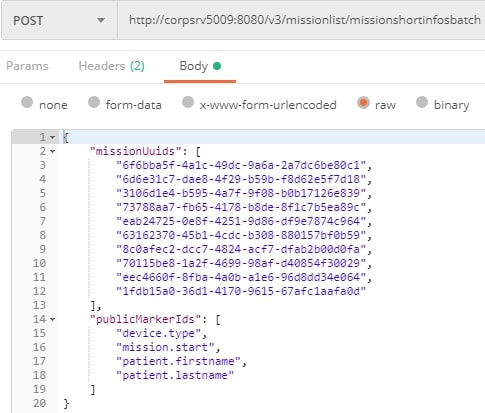
\includegraphics[width=.95\linewidth]{img/exRequestW}  
  \caption{Beispiel des POST-Requests}
  \label{fig:request}
\end{subfigure}
\begin{subfigure}{.5\linewidth}
  \centering
  % include second image
  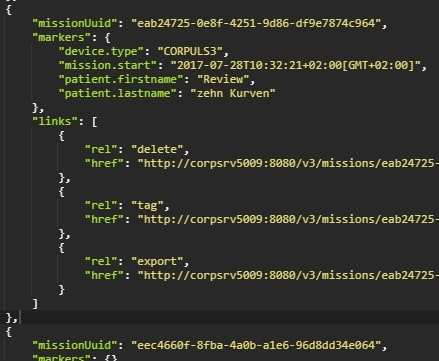
\includegraphics[width=.95\linewidth]{img/exResponse}  
  \caption{Auszug der Antwort auf den POST-Request}
  \label{fig:response}
\end{subfigure}
\caption[Beispiel einer Anfrage und Antwort der POST-Methode]{Beispiel einer Anfrage und Antwort der POST-Methode, um die \gls{MM} der im Body angegebenen Einsätze zu erhalten}
\label{fig:fig}
\end{figure}

In Abbildung \ref{fig:request} ist ein solcher POST-Request zu sehen.
In der URL wird der entsprechende \gls{ANALYSE}-Server adressiert, um auf die Daten der einzelnen Einsätze zugreifen zu können.
Im Body werden hierbei die aus Schritt 1 angeforderten Objekte eingefügt: \glqq missionUuids\grqq{} und \glqq publicMarkerIds\grqq.

Als Antwort erhält man mehrere \glqq Missions-Objekte\grqq{}, welche die \gls{UUID} und die entsprechenden \gls{MM} mit den individuellen Werten einer Mission enthält.
Ein Auszug einer solchen Antwort ist in \ref{fig:response} zu sehen.
Des Weiteren gibt es ein \glqq Link-Objekt\grqq{}, mit welchem ein Einsatz gelöscht, exportiert oder verändert werden kann. 

Positiv an diesem Export ist, dass die Anzahl der exportierten bedingt festgelegt werden kann.
Allerdings wird dieses Schema bei größeren Datenmengen, was genau das Ziel bei den Auswertungen ist, zu Problemen führen.
So kann das entsprechende Objekt mit den Einsatz-\gls{UUID}s sehr groß werden und beim kopieren und einfügen in den darauffolgenden Request-Body Schwierigkeiten bereiten.
Auch der damit resultierende große POST-Befehl ist keine optimale Umsetzung.

Aus diesem Anlass muss dieses Export-Format neu überdacht und für große Datenmengen optimiert werden.

\subsubsection{Überarbeitetes Export-Format}
\label{subsub:ueberarbeutetesformat}
Der Hauptaspekt beim neuen Entwurf der Export-Schnittstelle war das effiziente und sichere Umgehen mit großen Datenmengen.
Hierfür muss ein anderer als der zweistufige, in \ref{subsub:1stexport} beschriebene Prozess, entwickelt werden.

%\todo{Alternativen: Direkt auf Platte, Anstoßen und direkt Ergebnis erhalten oder eben Anfrage und später fertige Datei\\Warum letzteres: Nie Timeout und sicherheit(auth) und universell}
%\lipsum*[104]

Letztendlich wurde sich für ein/das Konzept mit den folgenden möglichen Schritten entschieden:
\begin{enumerate}
\item Die Generierung eines Exports anstoßen
\item Alle angeforderten Exports auflisten
	\begin{enumerate}
	\item Details zu einem explizitem Export bekommen
	\item Bestimmten Export löschen
	\end{enumerate}
\item Objekt/Datei mit allen Einsätzen und zugehörigen Daten mittels eigenem Link abrufen
\end{enumerate} 

Zum Erhalt der Export-Datei sind alle drei Schritte notwendig, 2a) \& b) sind als optionale Funktionen verfügbar.
Auch hier ist bei allen Vorgängen eine entsprechende Authentifizierung notwendig, um entsprechende Aktionen anzustoßen oder Informationen zu erhalten.

\begin{enumerate}
\item \code{-POST http://10.97.3.109:8080/v3/exports}
\end{enumerate}
Der erste Vorgang ist hierbei der POST-Befehl, der auf dem entsprechenden Server die Generierung eines neuen Exports anstößt.
Dabei werden alle verfügbaren Einsätze mit allen vorhandenen \gls{MM} exportiert.
Dies wurde so festgelegt, da der Anwender in der Regel mit einem solchen Export alle Missionen erhalten möchte.
\ref{sub:incremental}
%Die Erweiterung um einen ressourcensparenden \glqq Incremental Load\grqq{} wird in \ref{sub:incremental} weiter betrachtet.

\begin{enumerate}[resume]
\item \code{-GET http://10.97.3.109:8080/v3/exports}
\end{enumerate}

Daraufhin ist es mit dem zweiten Schritt möglich, alle angestoßenen, laufenden und fertigen Exports aufzulisten.
Dabei wird mit der identischen URL die GET-Methode ausgeführt.
Hierbei werden pro Export zusätzliche Informationen bereitgestellt (siehe Abbildung \ref{fig:exportListWide}): 

%Die Start-Zeit (\glqq startTime\grqq) als UTC-Zeitstempel in Millisekunden, wann dieser Export angestoßen wurde.
%Analog der End-Zeitpunkt (\glqq endTime\grqq) wann dieser Export fertiggestellt wurde, die Anzahl Missionen, der jeweilige Status, ob angestoßen, laufend oder fertig, Links für weitere Optionen sowie die ID des Exports.

\begin{itemize}
\item Start-Zeit (\glqq startTime\grqq): UTC-Zeitstempel in ms, wann dieser Export angestoßen wurde
\item End-Zeit (\glqq endTime\grqq): UTC-Zeitstempel in ms, wann dieser Export fertiggestellt wurde
\item Anzahl der exportierten Einsätze (\glqq missions\grqq)
\item Status, ob angestoßen, laufend oder fertig
\item Links zu den weiteren Optionen
\item Die ID des Exports
\end{itemize}

\bild
{exportListWide}
{12cm}
{Antwort des Servers - Auszug der Auflistung von zwei fertiggestellten Exports als JSON-Objekte}
{Auflistung von Exports}

Demnach werden angeforderte Exports für eine ausgewählte Dauer gespeichert, was für unterschiedliche Szenarien ein Vorteil sein kann.
Auch die Möglichkeit, einen angeforderten Export wieder zu löschen ist eine hilfreiche Funktion, welche einen Server entlasten kann, sollten beispielsweise zu viele Exporte angefordert worden sein.
Der Status ist ebenfalls eine nützliche Information, welche den Empfang des fertigen Exports an ein \gls{BI}-Werkzeug erleichtern und garantieren kann.

\begin{enumerate}[resume]
\item \code{-GET http://10.97.3.109:8080/v3/exports/\{EXPORT\_ID\}/file}
\end{enumerate}

Im letzten Schritt wird der entsprechend bereitgestellte Link mitels GET-Methode aufgerufen.
Daraufhin erhält der Anwender den gesamten Export mit allen Einsätzen und den dazugehörigen \gls{MM} im JSON-Format. 
Ein Beispiel dieser Antwort ist Abbildung \ref{fig:exportFile} zu entnehmen.
\bild
{exportFile}
{9cm}
{Auszug des Exports mit allen Einsätzen und dazugehörige \gls{MM}}
{Auszug des Exports}

Der größte Vorteil dieses neuen Formats ist der Umgang mit großen Datenmengen.
Es müssen keine riesigen Objekte kopiert und eingefügt oder an eine andere Stelle weitergeleitet werden. 
Auch sind keine weiteren umständlichen Parameter notwendig. \\
Die URL wurde mit dem Schema \\
\colorbox[RGB]{240,240,240}{\texttt{http://\{SERVER\_IP\}/v3/exports}} \\
standardisiert, sodass keine unterschiedlichen URLs mit vielen optionalen Parametern wie in \ref{subsub:1stexport} notwendig sind.
Lediglich beim finalen Anfordern der Export-Datei muss die Standard-URL um \\
\colorbox[RGB]{240,240,240}{\texttt{http://\{SERVER\_IP\}/v3/exports\textcolor{red}{/\{EXPORT\_ID\}/file}}} \\
erweitert werden. 

\subsection{Erweiterung um neue Datenobjekte} %tiefgreifendere? Daten}
\label{sub:erweiterung}
Im Rahmen der \fullref{kap:anforderungsanalyse} kamen bereits erste Fragestellungen zum Vorschein, welche mit den bisherig zur Verfügung stehenden Daten nicht beantwortbar waren.
Im darauffolgenden Laufe der \fullref{kap:konzept} haben sich diverse weitere Problematiken und fehlende Daten für aussagekräftige Auswertungen bestätigt.

So ist beispielsweise eine ausdrucksvolle Analyse zur Drucktiefe in der Reanimation über mehrere Missionen nicht in der Form umsetzbar, wie sie sinnvoll und gewünscht wäre.
Hier ist lediglich der Mittelwert der Drucktiefe von der gesamten Reanimation vorhanden.
Eine inhaltsreiche Auswertung, auch beispielsweise mit Veränderungen innerhalb der Reanimation, sind schlicht nicht möglich.
In diesem Stil gibt es weitere, für Auswertungen sinnvolle Daten, die derzeit gar nicht, oder nur als stark aggregierte Werte vorhanden sind.
Eine Analyse der potentiell verfügbaren Daten ergab folgende Bereiche (Auszug im Anhang \ref{anhangProbleme}):  %Markante Beispiele sind:
\begin{description}
\item [Reanimationsqualität]\hfill \\
Drucktiefe \& -frequenz, Anzahl Kompressionen, Pausenzeiten und \gls{CCF}
\item [Defibrillationen]\hfill \\
Zeitpunkt, Energie, Impedanz, Modus und Pausenzeiten der einzelnen Defibrillationen
\item [\gls{NIBD}]\hfill \\
Zeitpunkt, Modus, Dauer , Patiententyp, Systole, Diastole \& mittlerer arterieller Druck der einzelnen Messungen
\item [Vitalparameter und Trends]\hfill \\
Die Werte aller Vitalparameter zu einem bestimmten Zeitpunkt
\item [Technische- und Patienten-Alarme]\hfill \\
Wann sind welche Patientenalarme mit welchen Alarmgrenzen aufgetreten? \\
Welche technischen Alarme treten zu welcher Zeit auf?
\item [Events]\hfill \\
Welche Events treten wann mit welchen Parameter-Werten auf?
\end{description}

Mit diesen Daten wären weit detailliertere und tiefgreifendere Auswertungen möglich. 
Dabei würde vor allem die explorative Datenanalyse (siehe S.\pageref{subsub:datenanalyse}, \ref{subsub:datenanalyse}) profitieren.

Diese erfordern jedoch eine Überlegung des späteren Datenmodells, da diese das Konzept von multidimensionale Daten darstellen.
Demnach gibt es einen Datensatz mit \textit{n} Einsätzen, wovon jeder Einsatz eine Anzahl \textit{m} Kompressionen, Defibrillationen, Messungen, Alarme und weiteres haben kann.
Einen Entwurf für ein passendes Datenmodell ist in Abbildung \ref{fig:ersterVorschlagDatenmodellC} zu sehen.

Auf Basis dieser Analyse und der herausgefundenen potentiellen neuen Datenquellen werden Anforderungen formuliert und mit der Entwicklungsabteilung kommuniziert, damit diese Daten zur Auswertung bereitstehen können.

\subsubsection{Entwurf für ein Datenmodell}
\label{subsub:datenmodell}
Um die Anforderung, weitere Daten aus den bisherigen Einsätzen auszulesen gerecht zu werden, muss vorab ein geeignetes Datenmodell entworfen werden.
Dieses muss die daraus resultierende Multidimensionalität unterstützen und eine konfliktfreie Umgebung schaffen.
Dabei sollen jedoch so viele Daten wie möglich miteinander kombiniert werden können, damit ein umfassendes exploratives und konfirmatives Analysieren der vorliegenden Daten möglich ist.

Zuvor gab es lediglich die Tabelle \glqq Missions\grqq{}, welche pro Zeile einen Einsatz ablegt und in den dazugehörigen Spalten die Werte zu den entsprechenden \gls{MM}.
Ein Auszug aus hieraus ist in Tabelle \ref{tbl:missions} zu sehen.

\begin{table}[htb]
\centering
%\resizebox{\textwidth}{!}{%
\begin{tabular}{|l|l|l|l|l|}
\hline
\textbf{mission.uuid}   & \textbf{mission.start} & \textbf{hasReanimation} & \textbf{device.type} & \textbf{...} \\ \hline
b14f790f-{[}...{]}863f3 & 2016-08-27T12:13:07    & true                    & corpuls3             & ...          \\ \hline
d7276b88-{[}...{]}2da61 & 2016-09-29T21:02:30    & false                   & corpuls1             & ...          \\ \hline
\end{tabular}%
%}
\caption[Aktuelle Export-Tabelle]{Auszug aus der Tabelle, wie sie im aktuellen Export maximal zur Verfügung steht}
\label{tbl:missions}
\end{table}

Ein geeignetes Datenmodell, welches die mehrdimensionalen Daten einbindet und unterstützt, wurde entworfen und ist in Abbildung \ref{fig:ersterVorschlagDatenmodellC} zu erkennen.
Hierbei wurden die in \ref{sub:erweiterung} genannten neuen Datenquellen hinzugefügt, sodass beispielsweise neue Tabellen zu \gls{CPR}- oder Defibrillationsdaten zu sehen sind.

\bildbreit
{ersterVorschlagDatenmodellC}
{Visualisierung für den Entwurf eines neuen Datenmodells mit mehrdimensionalen Objekten}
{Visualisierung des neuen Datenmodells mit mehrdimensionalen Objekten}

Dabei wurde darauf geachtet, dass keine zirkulären Referenzen entstehen, welche unter anderem bei der gleichen Benennung mehrerer Spalten vorkommen.
Dies wurde präventiv mit einem Präfix der jeweiligen Datenquelle verhindert.
Auch erleichtert dies das spätere Erstellen von Dimensionen oder Kennzahlen, da eine eindeutige Benennung vorhanden ist.

Auch ein gemeinsamer Primärschlüssel sollte in allen neuen Datentabellen vorhanden sein, damit eine Beziehung herrscht.
Hierfür wurde die \gls{UUID} verwendet, da diese garantiert in jedem Einsatz vorhanden und bereits eindeutig ist.
Damit ist gewährleistet, dass theoretisch jeder Datenpunkt mit jedem anderen Datenpunkt verknüpft werden kann, auch wenn nur ein geringer Teil aller Verknüpfungen sich als sinnvoll erweisen wird. 


%\subsection{Incremental Load?}
\subsubsection{Erstellen von Anforderungen für neue Datenquellen} %(als User Stories in JIRA)}
\label{subsub:stories}
Damit die im vorherigen Kapitel herausgefundenen Datenquellen für Auswertungen bereitstehen, muss zunächst deren Extrahierung aus den Einsatzdaten implementiert werden. 
Weiter steht der Export, beziehungsweise das Hinzufügen dieser neuen Daten in den bestehenden, überarbeiteten Export an.

Hierfür wird der bestehende Prozess der Entwicklungsabteilung angewandt, damit eine entsprechende Implementierung im SCRUM-Verfahren möglich ist.
Demnach wird für eine neue Anforderung eine \glqq Story\grqq{} im Projekt- und Aufgabenmanagement-Tool \glqq Jira\grqq{} angelegt.
Diese Story wird einem übergeordneten \gls{Feature} oder \glqq Epic\grqq{} zugeordnet.
So werden beispielsweise dem Feature \glqq \gls{BI} Dashboard\grqq{} alle zugehörigen Storys zugeordnet, wie in einem Auszug davon in Abbildung \ref{fig:jiraEpic} zu sehen ist.
\bild
{jiraEpic}
{12cm}
{Grafische Visualisierung der zugehörigen Storys vom Feature \glqq \gls{BI} Dashboard\grqq{} in Jira}
{Visualisierung der zugehörigen Storys vom Feature BI-Dashboard in Jira}

Weiter muss eine Story laut SCRUM die \glqq Definition of Ready\grqq{} erfüllen, damit sie in den Sprint mit eingeplant werden darf.
Diese soll garantieren, dass unter anderem eine aussagekräftige Beschreibung oder Abnahmekriterien vorhanden sind.
Dementsprechend müssen die erstellten Storys gewisse Qualitätsmerkmale vorweisen, damit sie umgesetzt werden können.

Für das Extrahieren und Exportieren von einem neuen Datenobjekt ist es daher sinnvoll, die geforderten Informationen so detailliert wie möglich darzulegen.
Hierfür ist das vorab in \ref{subsub:datenmodell} entwickelte Datenmodell ein hilfreiches Mittel, um die Storys präzise beschreiben zu können.

\begin{table}[hbt]
\centering
\resizebox{\textwidth}{!}{%
\begin{tabular}{ll|l|l|l|l|l|l|}
\cline{3-8}
                                       &                       & \multicolumn{6}{c|}{\textbf{trend.}}                                                                                                                                              \\ \cline{3-8} 
                                       &                       &                       & \multicolumn{5}{c|}{\textbf{cpr.}}                                                                                                                        \\ \hline
\multicolumn{1}{|l|}{\textbf{}}        & \textbf{mission.uuid} & \textbf{minute} & \textbf{pauses.sum} & \textbf{comp.sum} & \textbf{depth.avg} & \textbf{rate.avg} & \textbf{ccf} \\ \hline
\multicolumn{1}{|l|}{\textbf{Type}}    & uuid                  &                       & int                           & int                                 & float                        & float                       & float                  \\ \hline
\multicolumn{1}{|l|}{\textbf{Unit}}    &                       &                       & s                             &                                     & cm                           & 1/min                       &                        \\ \hline
\multicolumn{1}{|l|}{\textbf{Example}} & sd84-[...]-k9s4s      & 3                     & 13                            & 91                                  & 5.31                         & 112                         & 0.82                   \\ \hline
\end{tabular}%
}
\caption[Gefordertes Exportformat am Beispiel der CPR-Daten]{Auf Basis des entworfenen Datenmodells erstellte Tabelle für das geforderte Export-Format am Beispiel von \gls{CPR}-Daten}
\label{tbl:export}
\end{table}

Für eine solche detaillierte Beschreibung der Story wurde unter anderem eine Tabelle \ref{tbl:export} angelegt.
In dieser Darstellung sind bereits viele Aspekte festgelegt.
So ist beispielsweise die Namensgebung an die bisherige Nomenklatur der \gls{MM} angelehnt, sodass eine innere Konsistenz herrscht.
Auch der jeweilige Datentyp oder die Einheit ist bereits festgelegt, damit ein einheitliches Format der Daten gewährleistet ist.

Die Einheit ist insofern von großer Bedeutung, da diverse Daten in verschiedenen Einheiten gespeichert werden können.
So kann etwa die CO2-Konzentration der Ausatemluft in Millimeter-Quecksilbersäule (mmHg) oder Kilopascal (kPa) gemessen und gespeichert werden.
Damit in der späteren Auswertung keine unterschiedlichen Einheiten vermischt werden, wird in Tabelle \ref{tbl:export} eine Standard-Einheit für den Export festgelegt.

Auch der Aggregierungsgrad wird hier beschrieben, indem die Daten für eine Minute aggregiert werden sollen.
Dies resultierte aus mehreren Diskussionen mit Entwicklern, Produktmanager und Stakeholdern, da die Speicherung von jeder einzelnen Kompression mit ihren vorliegenden Daten auf lange Sicht zu einem Speicher- und Performanceproblem führen könnte.
Dennoch ist es für die Anwender eine deutliche Verbesserung der Auswertungsmöglichkeiten.

Ein Beispiel für exemplarische Daten wird ebenfalls hinzugefügt, damit letzte Unklarheiten zu Feldern oder Datentypen beseitigt werden.
Dieser Prozess wird analog mit allen neu geforderten Objekten (siehe Abbildung \ref{fig:ersterVorschlagDatenmodellC}) durchgeführt. Anhang jira stories\ref{AnhangJiraStories?}

\subsubsection{Festlegen des Export-Formats}
Im Zuge der Bereitstellung der neuen Datenobjekte wurde im vorigen Kapitel mittels Beschreibung der Anforderungen und ergänzenden Tabellen das gewünschte Format festgelegt.
Im Laufe der Implementierung gibt es diverse Diskussionen und Abstimmungen mit den Entwicklern und Stakeholdern, wie der finale Export aussehen soll.
Dies geschieht im Zuge der \glqq Sprints\grqq{} in mehreren Zyklen, wird jedoch für die bessere Lesbarkeit dieser Arbeit in diesem Unterkapitel zusammengefasst.

Vorab ist anzumerken, dass im zeitlichen Rahmen dieser Arbeit und unter Berücksichtigung von anderen Entwicklungsprojekten eine Priorisierung des Product-Owners vorgenommen werden musste.
Dabei sind drei der sechs geforderten neuen Datenobjekte aus Abbildung \ref{fig:ersterVorschlagDatenmodellC} für die Erweiterung des Exports  geplant: \gls{CPR}-, \gls{NIBD}- \& Defibrillations-Daten.

Demnach soll es drei optionale neue JSON-Objekte in der Antwort des Servers (siehe Abbildung \ref{fig:exportFile}) geben.
Hier wurden vorab Überlegungen getätigt, wo die entsprechenden neuen Daten hierarchisch zugeordnet werden.
Dabei gibt es generell zwei Optionen:
Die neuen Objekte dem \glqq markers\grqq-Objekt unterordnen (Abbildung \ref{fig:marker}), oder direkt unterhalb des \glqq mission\grqq-Objektes als zweiten Kindknoten (\ref{fig:mission}).

\begin{figure}[ht]
\begin{subfigure}{.5\linewidth}
  \centering
  % include first image
  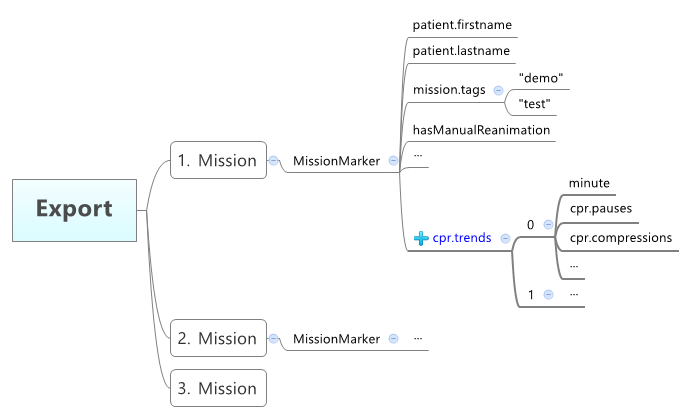
\includegraphics[width=.95\linewidth]{img/format1}  
  \caption{CPR-Objekt unterhalb des \glqq markers\grqq-Objekt}
  \label{fig:marker}
\end{subfigure}
\begin{subfigure}{.5\linewidth}
  \centering
  % include second image
  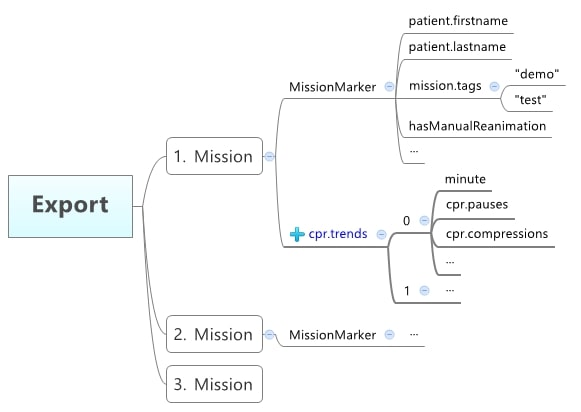
\includegraphics[width=.95\linewidth]{img/format2}  
  \caption{Neues Objekt neben dem \glqq markers\grqq-Objekt}
  \label{fig:mission}
\end{subfigure}
\caption[Beispiel einer Anfrage und Antwort der POST-Methode]{Schematische Darstellung der Erweiterung des Exports am Beispiel vom CPR-Objekt}
\label{fig:tree}
\end{figure}

Da es sich um eigenständige neue Objekte unabhängig von den \gls{MM} handelt, wurde sich für die Variante in Abbildung \ref{fig:mission} entschieden.
Demnach können nun die Objekte \glqq trend.cpr\grqq, \glqq shock.details\grqq{} und \glqq nibp.details\grqq{} in einem Missions-Objekt vorhanden sein.
Ein Beispiel hierfür ist in Abbildung \ref{fig:exportNewObj} zu sehen.

\bild
{exportNewObj}
{9cm}
{Neue JSON-Objekte (hier \glqq trend.cpr\grqq{} \& \glqq shock.details\grqq{}) neben den \glqq markes\grqq{} innerhalb eines Missions-Objektes des Exports}
{Neue JSON-Objekte innerhalb eines Missions-Objektes des Exports}

%(Diese zwei Optionen sind in Abbildung \ref{fig:tree} schematisch dargestellt.
%Dabei ist in \ref{fig:marker} das Schema mit der Unterordnung unterhalb des \glqq markers\grqq-Objekt visualisiert.
%In \ref{fig:mission} ist das \gls{CPR}-Objekt unterhalb der ersten Mission als zweites Kindobjekt neben den \glqq markers\grqq angelegt.)

Des Weiteren wurde entschieden, die neuen Objekte nur zu exportieren, wenn auch tatsächlich Daten hiervon vorhanden sind.
Bei dem \gls{CPR}-Objekt gibt es hierbei eine Besonderheit, da dieses als zeitliches Objekt mit Trenddaten anzusehen ist.
Dadurch gibt es immer Daten ab Minute 0, auch wenn beispielsweise die erste Kompression erst in Minute zwölf stattfand.
Dies soll garantieren, dass eine kontinuierliche Zeitskala gegeben ist, die auch mit anderen Trenddaten vergleichbar ist.
Für eine Vergleichbarkeit von Reanimationen untereinander ist diese Form der Daten nicht geeignet. 
In \ref{subsub:weitereFelder} wird eine Lösung erarbeitet, die dies zusätzlich ermöglichen soll.

Bei den \gls{NIBD}- \& Defibrillations-Objekten ist im Gegensatz zum CPR-Objekt nicht die Minute das führende Feld respektive Primärschlüssel, sondern die hochzählende Nummer der Messung oder der Schockabgabe.
Dadurch ist aufgrund der Objekorientierung eine Repräsentation der Wirklichkeit gegeben, da eine Messung oder eine Defibrillation ein abgeschlossenes Objekt darstellt.

%(json format cpr (siehe mails) (Fotos whiteboard als anhang?),)
%null values bei cpr trends

%% Vor Export?
%\subsection{Datenbankhaltung?}
%\subsubsection{Lasttests?}
%%dummydaten?


%\section{Datenmodell?}

\section{Erstellung der Qlik-App}
\label{sec:erstellung}
%subsUnterschiedliche Apps?
\subsection{ETL-Prozess}
\label{sub:etl}
Um Rohdaten aus einem Export in ein adäquates Format für spätere Auswertungen zu bringen, ist in der Regel ein \gls{ETL}-Prozess notwendig.
Dieser soll garantieren, dass ein einheitliches \gls{DWH}, wie in \ref{sub:warehouse} beschrieben, gegeben ist \cite[S.49]{Gabriel.2011}.
\todo{Bild ETL Prozess}

Das Extrahieren der Daten wird mittels eines \gls{REST}-Konnektors realisiert.
Dabei kann in der Qlik-Software oder im \gls{QMC} der Qlik-Enterprise Version eine Schnittstelle definiert werden, welche per REST einen Datenverbindung aufbaut.
Anschließend werden die extrahierten Daten mit Hinblick auf die zu beantwortenden Fragen (\ref{sec:erhebung}) transformiert.

Dabei ist die Besonderheit, dass zuerst die Generierung eines Exports getriggert werden muss und anschließend kann der fertige Export angefragt werden (siehe \ref{subsub:ueberarbeutetesformat}).
Dadurch entsteht die Notwendigkeit von zwei REST-Datenverbindungen, da eine Verbindung jeweils nur eine Methode (GET, POST) umsetzen kann.

Die Skripte, die diesen ETL-Prozess umsetzen, werden im Folgenden näher erläutert.

\subsubsection{Ladeskripte}
\label{subsub:scripts}
%\todotext{Datenverbindungen erklären? Skripte in Anhang?}

Um die Daten im entsprechend geforderten Format vorliegen zu haben, sind eine Reihe von \gls{ETL}-Prozessen notwendig.
Diese wurden mittels der eigenen Skriptsprache von Qlik angefertigt (siehe \ref{sub:qlik}).

Dabei wurde eine logische Unterteilung in sechs Abschnitte vorgenommen.
Abschnitt 1 kann hierbei dem Extrahieren und die Abschnitte 2-5 dem Transformieren der Daten gleichgesetzt werden.

Eine genauere Beschreibung der entsprechenden Skripte in deren Abschnitte kann nachfolgend eingesehen werden:
\begin{description}
\item[Abschnitt 0 - Präambel] \hfill \\
Hier werden diverse Konfigurationseinstellungen eingestellt.
Darunter fällt beispielsweise die Festlegung des Datums-, Zeit- oder Währungsformats, Abkürzungen und weitere Länderspezifische Einstellungen.

Des Weiteren werden Mapping-Tables erstellt, welche später generische Benennungen der Daten seitens der Geräte in verbesserter Form darstellen sollen. 
Beispiel: CORPULS\_WEB\_LIVE - corpuls.web LIVE

\item[Abschnitt 1 - Extrahieren der Daten]  \hfill \\
Die folgenden Skripte wurden als ersten Abschnitt deklariert, da sie den ersten Prozess von \gls{ETL} realisieren.
Demzufolge wird nach den Methoden in \ref{subsub:ueberarbeutetesformat} zuerst die Erzeugung eines Exports angefordert.
Daraufhin wird per Skript aus dem Header der Server-Antwort die entsprechende URL extrahiert, welche auf den erzeugten Export verweist.
Diese URL wird um das Suffix \code{/file} ergänzt und in einer Variable gespeichert.
Abschließend wird der neue Export mit dieser URL per SQL-Select-Befehlen angefordert.

\item[Abschnitt 2 - Missionen laden und filtern] \hfill \\
Dieser Abschnitt ist der Beginn des Transformieren der extrahierten Daten.
Dabei wird als erster Schritt eine begrenzte Anzahl an \gls{MM} geladen, mittels welcher eine Filterung von Test-Einsätzen möglich ist.
Diese Filterung wird in \ref{subsub:testfilter} näher beschrieben.

Anschließend werden auf Basis der herausgefilterten Einsätze nur jene geladen, die nach diesem Schritt als relevant angesehen werden.
Dabei werden zuerst alle verfügbaren \gls{MM} geladen, da jeder Einsatz MM enthält und folglich eine 1:1 Beziehung herrscht.
Hier werden auch bereits weitere Felder hinzugefügt, welche für spätere Auswertungen benötigt werden.
Auf diese wird in \ref{subsub:weitereFelder} weiter eingegangen.

Auch die zugehörigen \glqq Mission-Tags\grqq{} werden in diesem Abschnitt geladen und in Relation mit der zugehörigen Mission gesetzt.
Außerdem werden jene Einsätze in einer Tabelle festgehalten, die als \glqq Test\grqq{} klassifiziert wurden, um spätere Informationen zu diesen zur Verfügung stellen zu können.

\item[Abschnitt 3 - Weitere Datenobjekte laden, bearbeiten und verknüpfen] \hfill \\
Das Laden der Objekte, die in \ref{sub:erweiterung} erarbeitet wurden, ist als 3. Schritt kategorisiert.
Demnach werden die bis zu diesem Zeitpunkt der Umsetzung verfügbaren neuen Objekte geladen: \gls{CPR}, Defibrillation und \gls{NIBD}.

Zur Reduzierung der Laufzeit werden hier mittels JOIN-Befehle nur jene Objekte geladen, die einem Einsatz zugehörig sind, welcher nicht als \glqq Testeinsatz\grqq{} eingestuft wurde.
Dadurch wird außerdem die Verzerrung der Daten ausgeschlossen beziehungsweise minimiert.

Auch hier werden weitere Felder für spätere Auswertungen erzeugt.
Außerdem werden die Daten mittels der in Abschnitt 0 erstellten Mapping-Tabellen harmonisiert und weitere Verbesserungen wie beispielsweise Rundungen vorgenommen, um ein einheitliches \gls{DWH} aufzubauen.

\item[Abschnitt 4 - Faktentabelle erstellen] \hfill \\
Um das in \ref{sub:datenmodell} beschriebene Datenmodell umzusetzen, wird hier eine Faktentabelle angelegt.
Dabei werden alle Objekte aus den Abschnitten 2 \& 3 mit unterschiedlichen JOIN-Befehlen zusammengeführt.
Dies garantiert die Realisierung des gewünschten Datenmodells.

\item[Abschnitt 5 - Sonstige Funktionen] \hfill \\
Als finalen Abschnitt werden jene zusätzliche Skripte zusammengefasst, welche weitere Funktionen umsetzen.
Ein Beispiel hierfür ist der \glqq Autocalender\grqq{} von Qlik Sense.
Dadurch ist beispielsweise die Darstellung von Liniendiagrammen über mehrere Jahre optimiert.
\todotext{bildvergleich mit ohne autocalendar?}
\end{description}

\subsubsection{Demo- und Testeinsätze herausfiltern}
\label{subsub:testfilter}
Um eine hohe Qualität der entsprechenden Auswertungen gewährleisten zu können, ist das Filtern von irrelevanten Einsätzen ein essentieller Schritt.
Da auf den Auswertungen diverse Entscheidungen getroffen werden können, die von Materialplanung über Ressourcenbeschaffung bis hin zu Schulungsmaßnahmen reichen, ist eine möglichst unverfälschte Darstellung der relevanten Daten notwendig.

Hierfür müssen gewisse Kriterien festgelegt werden, die einen Einsatz als nicht relevanten Einsatz einstufen.
Eine weitere Überlegung hierbei wäre, je nach zutreffenden Kriterien eine Wahrscheinlichkeit für einen Testeinsatz anzugeben.
Dieser Ansatz ist im Rahmen dieser Arbeit aufgrund des größeren Umfangs nicht weiter verfolgt worden, sollte jedoch für die weitere Planung berücksichtigt werden.

Kriterien die in dieser Umsetzung verwendet wurden sind unter anderem das Anschließen einer Test-Box, verschiedene Test-Modi des \gls{cAED}, unrealistisches Datum (2000 > Jahr > 2020) oder eine zu kurze oder deutlich zu lange Einsatzdauer.

Diese Kriterien können beliebig von einem entsprechend berechtigtem Anwender oder Entwickler im Abschnitt 2 der Ladeskripte erweitert oder eingeschränkt werden.
Es wird darüber hinaus dem Anwender noch eine weitere Möglichkeit des Herausfilterns gegeben.
Dies geschieht über die Erweiterung der alten Filterleiste (siehe S. \pageref{par:filter}) um das Dropdown-Filterfenster \glqq Mission-Tags\grqq{} in den entsprechenden Dashboards. %\todotext{(Dazu in ref() mehr)}
Dadurch ist eine 100\%-Filterquote von Testeinsätzen realisierbar, sofern die sinngemäße Verwendung der Mission-Tags angewandt wird.

\subsubsection{Erweiterung um manuell hinzugefügte Felder}
\label{subsub:weitereFelder}
Im Zuge der iterativen Entwicklung und in Anbetracht der zu beantwortenden Fragestellungen stellt sich heraus, dass die zugrundeliegenden Daten nicht ausreichend genug oder zu detailliert sind.
Hierfür können im \gls{ETL}-Prozess weitere Felder manuell hinzugefügt werden, die in der Regel auf den vorliegenden Daten basieren.

Eine Auswahl an den neuen oder veränderten Feldern sind beispielsweise gerundete Trend- oder Messdaten wie die Konvertierung der Kompressionstiefe von \glqq Float\grqq{} zu einer Zahl mit einer Nachkommastelle.
Auch entsprechend zusätzliche Datums- und Zeitdaten wurden auf der Basis der vorhandenen Daten generiert. 
So wurde alleine aus dem einen \gls{MM} \glqq mission.start\grqq{} eine Vielzahl an neuen Feldern erzeugt, anhand welcher neue genauere oder aggregiertere Auswertungen möglich sind: Wochentag, Stunde, Stundenfenster, Minute oder Tagesabschnitt.

Auch manuelle Klassen von Werten wurden beispielsweise bei der Kompressionstiefe oder -frequenz des neuen Datenobjektes erstellt, da sich in der Evaluation des Prototyps herausstellte, dass es irrelevant ist, ob eine Kompression 1,2cm oder 1,6cm tief war (siehe S.\pageref{par:binning}).
Viel interessanter ist die Anzahl der Kompressionen die mit 1-3cm deutlich zu flach, 4-5cm leicht zu flach und 5-6cm ideal waren.

Ebenso das Hinzufügen des Feldes \glqq Reanimations-Minute\grqq{} ist eine wichtige Berechnung, welche den Vergleich von mehreren Reanimationen überhaupt erst ermöglicht.
Dabei wird die Minute der ersten eintretenden Kompression bei jedem Einsatz als erste \glqq Reanimations-Minute\grqq{} abgespeichert. 

\subsection{Datenmodell}
\label{sub:datenmodell}
Im Laufe der Entwicklung wurden diverse unterschiedliche Datenmodelle ausprobiert.
Dementsprechend war auch das in \ref{subsub:datenmodell} konzeptionierte Datenmodell aus Abbildung \ref{fig:ersterVorschlagDatenmodellC} zwischenezitlich umgesetzt.
Jedoch stellte sich heraus, dass dieses Modell eine große Tabelle abbildet.
Dadurch war keine gute Trennung der Daten und folglich eine verschlechterte Performanz zu spüren.

Darausfolgend wurden unterschiedliche Datenmodelle umgesetzt und getestet, um die bestmögliche Effizienz aus Speicherbedarf und Performanz zu erlangen.
Hierbei gibt es die zwei Schemata \glqq Star\grqq{} \& \glqq Snowflake\grqq{} zur Umsetzung der Klassifikationshierarchie \cite{Kimball.2013}.
Die Namensgebung resultiert aus der visuellen Anordnung der Datentabellen, welche in Abbildung \ref{fig:compScheme} zu erkennen ist.

\begin{figure}[ht]
\begin{subfigure}{0.5\linewidth}
  \centering
  % include first image
  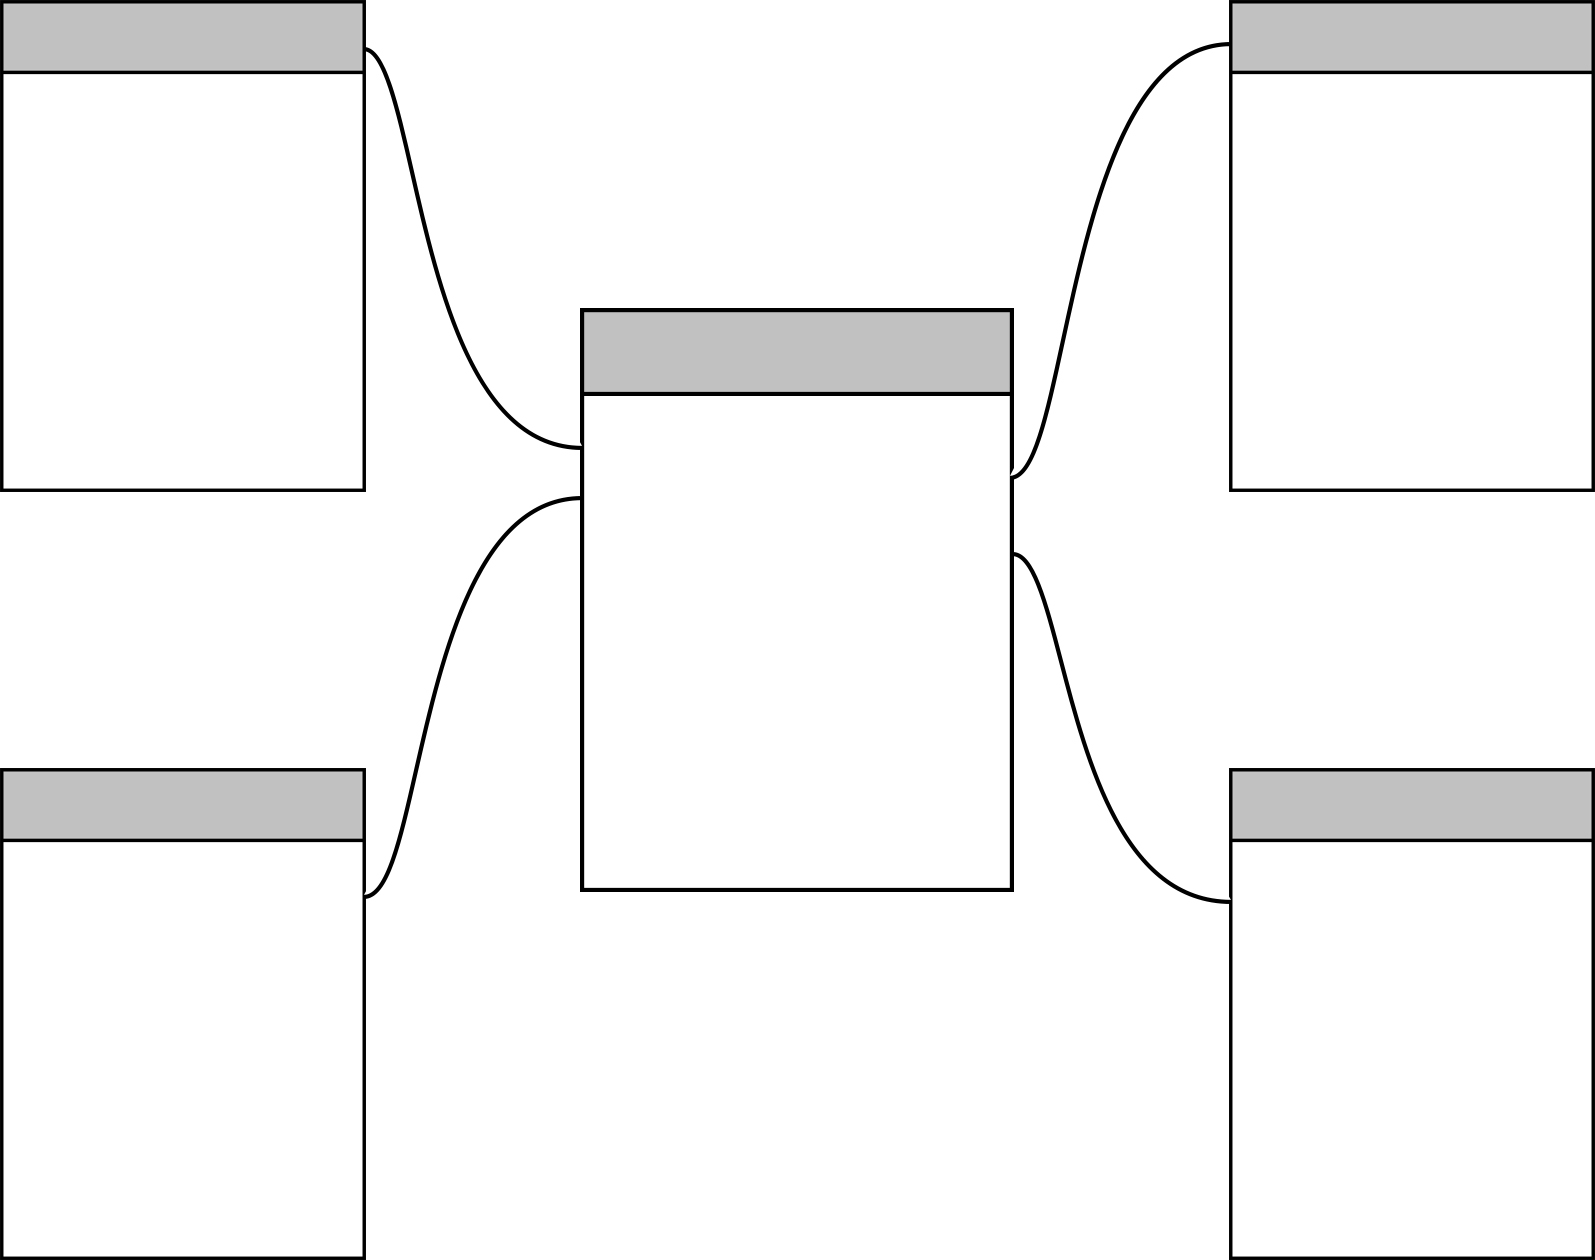
\includegraphics[width=0.95\linewidth]{img/starScheme}  
  \caption{Beispiel des Star-Schemas. Eine Faktentabelle mit Dimensionstabellen}
  \label{fig:starscheme}
\end{subfigure}
\begin{subfigure}{0.5\linewidth}
  \centering
  % include second image
  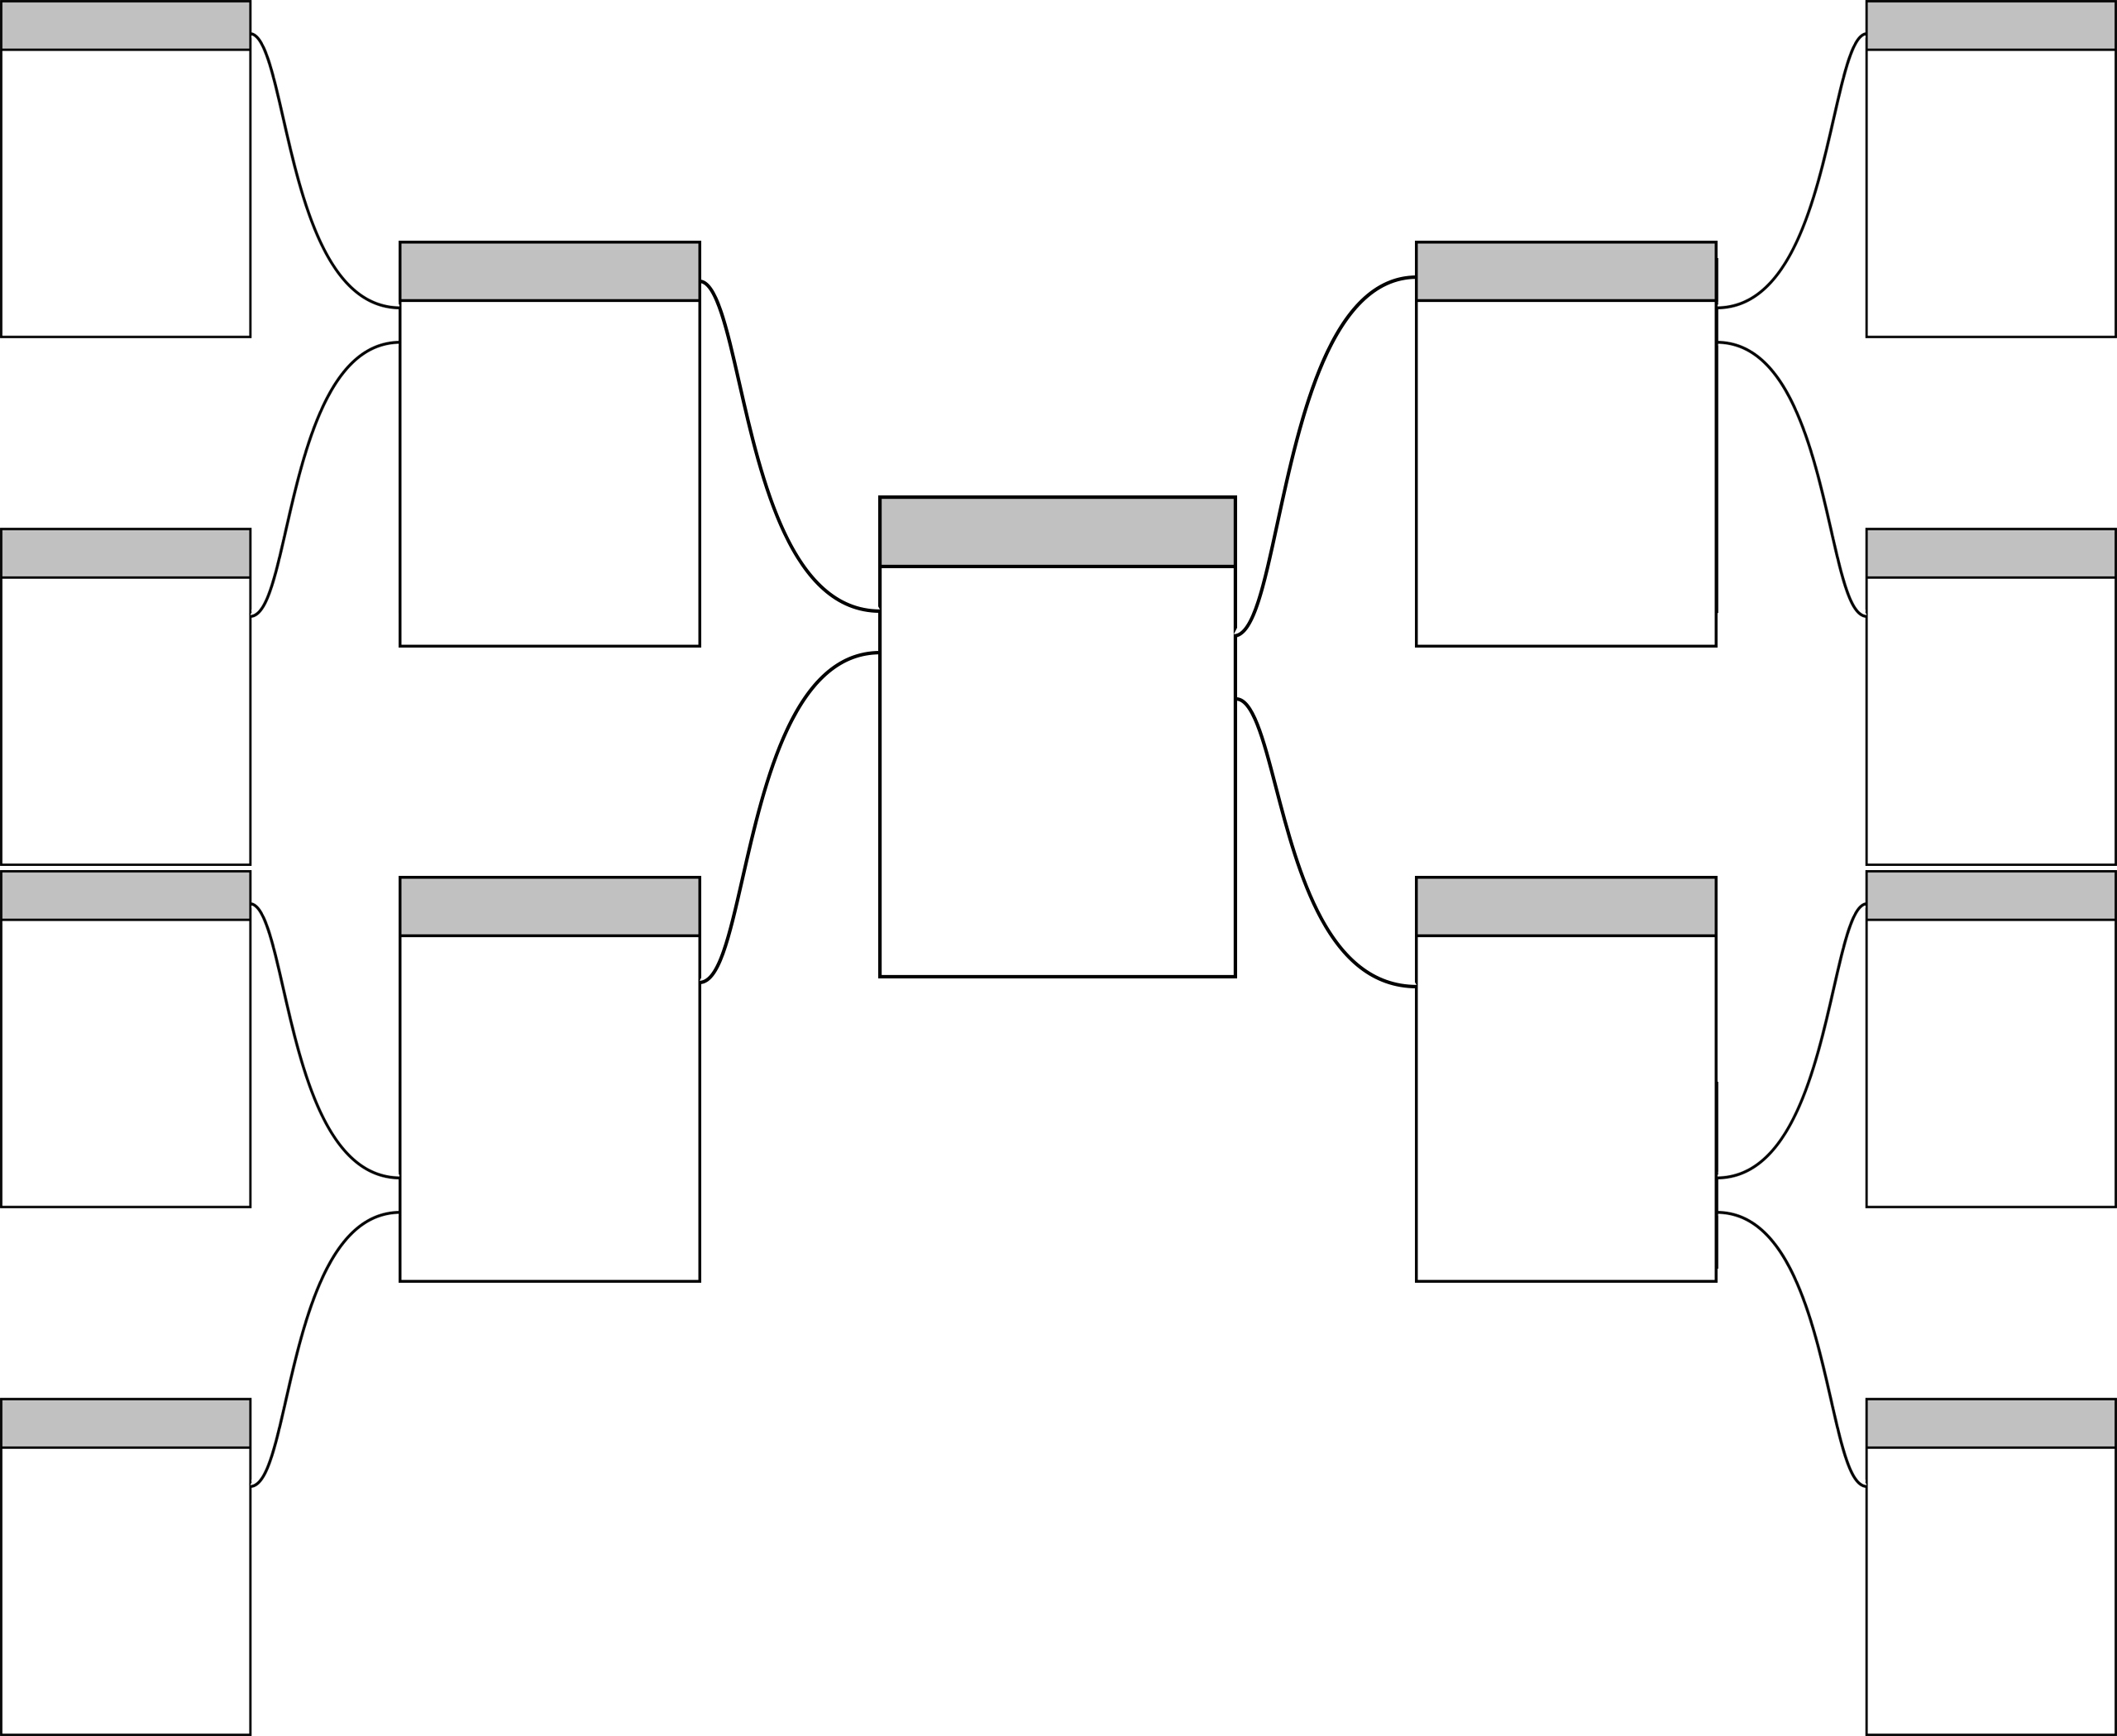
\includegraphics[width=0.95\linewidth]{img/snow}  
  \caption{Snowflake-Schema, welches weitere Dimensionstabellen beinhaltet}
  \label{fig:snow}
\end{subfigure}
\caption[Vergleich des Star- und Snowflake-Schemas]{Vergleich der beiden Schemata zur Umsetzung von Datenmodellen. Links Star, rechts Snowflake}
\label{fig:compScheme}
\end{figure}

%\bild
%{compStarSnow}
%{8cm}
%{Visuelle Darstellung des Star- und Snowflake-Schemas \todo{bildquelle!, vermutlich eigene Darstellung}}
%{Visuelle Darstellung des Star- und Snowflake-Schemas}

Demnach wurde als nächstes das Modell in ein Snowflake-Schema mittels verschiedener Befehle konvertiert. 
Nach einer kurzen Erprobung dieses Schemas stellte sich jedoch heraus, dass die Normalisierung, wie sie bei diesem Konzept vorgesehen ist, bei den vorliegenden Daten keinen großartigen Mehrwert bietet.
Die Einschränkungen in der Performanz und kompliziertere Abfragemechanismen gegenüber der Einsparung von Speicherplatz hat sich ebenfalls als nicht lohnenswert herausgestellt.

Aufgrund dieser Erkenntnisse wurde sich letztendlich für das Star-Schema entschieden.
Dieses Konzept zeigt Stärken in der Performanz durch Redundanzen in den entsprechenden Tabellen \cite[6.1]{Bauer.2004}. 
Die dadurch resultierende größere Anforderung an Speicherbedarf ist in diesem Zusammenhang vernachlässigbar, da die zukünftigen Versionen auf Servern laufen werden, welche mit genügen Ressourcen die Datenmengen problemlos stemmen können.
Aufgrund der Lesbarkeit sind die in \ref{subsub:scripts} erläuterten Skripte bereits auf dieses Schema gerichtet. 
Eine Darstellung dieses umgesetzten Datenmodells im Star-Schema ist in Abbildung \ref{fig:star2} zu erkennen.

\bild
{star2}
{10cm}
{Umgesetztes Datenmodell als Star-Schema in der Qlik-App}
{Umgesetztes Datenmodell als Star-Schema in der Qlik-App}

Hierfür wurden eigene Primärschlüssel in den Dimensionstabellen vergeben, sodass ein Einsatz als ein Eintrag in der Faktentabelle \glqq missions\grqq{} abgebildet werden kann.

%\subsection{Dimensionen}
%\subsection{Kennzahlen}
\subsection{Verwendung von Erweiterungen}
\label{sub:extension}
Qlik Sense bietet eine breite Palette an Standard-Visualisierungen, die den größten Teil der Anforderungen der meisten Kunden abdecken.
Jedoch gibt es für manche Daten bessere Darstellungsvarianten, welche die Lesbarkeit oder Aussagekraft der Daten verbessert oder Funktionen, die standardmäßig nicht vorhanden sind.

Dementsprechend wurde auf den sogenannten \glqq Qlik Branch\grqq{} zurückgegriffen \cite{QlikTech.2019b}.
Dies ist eine Plattform für Entwickler, auf welcher diverse Ressourcen veröffentlicht und heruntergeladen werden können.
Dabei können im \glqq Garden\grqq{} Erweiterungen heruntergeladen werden, welche die Funktionalitäten erweitern oder weitere Diagrammtypen ermöglichen.
Die Einbindung dieser geschieht in der Desktop-Variante per Einfügen in den entsprechenden Ordner, bei der Enterprise-Version mittels Import als ZIP-Datei.

Für die Umsetzung der Qlik-App wurden im wesentlichen vier Erweiterungen verwendet.
Diese werden nachfolgend kurz erläutert:
\begin{description}
\item[Buttons] \hfill \\
Eine Funktionalität, um Buttons in den Dashboards zu integrieren, gibt es standardmäßig nicht.
Hierfür gibt es eine Erweiterung \glqq Navigations \& Actions\grqq{}, welche dies ermöglicht.
Dabei können beispielsweise bestimmte Filterungen vorgenommen werden.
Dies wurde in dieser App für das einfache Umschalten von Reanimationen verwendet.
Jedoch ist dies aufgrund der später entdeckten Funktionalität \glqq Lesezeichen\grqq{} (siehe \ref{subsub:lesezeichen}) obsolet.

Für etwaige Navigationselemente oder als Schalter für die Internationalisierung kann diese Erweiterung jedoch in Zukunft weiter verwendet werden.
\item[Container] \hfill \\
Diese Erweiterung namens \glqq ShowHide Container\grqq{} ermöglicht es, gewisse Master-Elemente mit Hilfe von Bedingungen zu verbergen oder anzuzeigen.
In diesem Beispiel wurde sie dafür verwendet, eine Detail-Tabelle nur dann anzuzeigen, wenn eine Filterung weniger als zehn Einsätze zur Konsequenz hat (siehe \ref{par:DetailTabelle}). 

\item[Heatmap] \hfill \\
Es gibt diverse Fragestellungen aus \ref{sec:erhebung}, bei welchen beispielsweise die Auslastung von einer Wache oder einem oder mehreren Geräten interessant ist.
Dies kann mit den Visualisierungen aus \ref{subsub:zeitpunkt} bereits weitestgehend beantwortet werden.
Jedoch ist unter anderem für die Schichtplanung eine Auslastung in einer Wochentags- und Uhrzeit-Kombination von hoher Relevanz.
So müsste bei den Diagrammen jeder Wochentag gefiltert werden und anschließend kann aus dem Balkendiagramm zu den Stunden eine Auslastung abgeleitet werden.
Dies bietet allerdings keinerlei Überblick und hierfür ist eine \glqq Heatmap\grqq{} eine sehr nützliche Darstellung.

\bild
{heatmap}
{10cm}
{Beispiel einer Heatmap mit einer Visualisierung von Einsätzen pro Wochentag und Uhrzeit}
{Heatmap Visualisierung von Einsätzen pro Wochentag und Uhrzeit}

Die Erweiterung \glqq 2-dimensional Heatmap\grqq{} kombiniert, wie der Name suggeriert, zwei Dimensionen und eine Kennzahl.
Dabei ist in Abbildung \ref{fig:heatmap} auch die farbliche Hervorhebung der quantitativ hohen Daten zu erkennen, was die Charakteristik einer Heatmap ist.

\item[Radar-Chart] \hfill \\
Als verbesserte Darstellung von zyklischen Daten bieten sich sogenannte Radar-Diagramme an.
Diese wurden bereits in der Konzeptionsphase eingebunden (siehe S. \pageref{fig:radar} Abbildung \ref{fig:radar}).
Somit ist beispielsweise die Anzahl an Einsätzen pro Stunde nicht mehr in einem Balkendiagramm mit einem Anfang und einem Ende, sondern so wie es das mentale Modell des Anwenders erwartet analog zu einer Uhr als zyklische Darstellung.
\end{description}


\section{Dashboards}
\label{sec:dashboard} %Golden Rules
Es gibt viele unterschiedliche Regelwerke für Dashboards.
Der Ursprung der meisten Regelwerke liegt vermutlich in den \glqq International Business Communication Standards (IBCS)\grqq{} \cite{Hichert.2017}.
Eine Auswahl dieser Regeln betreffen etwa die Anzahl an Elementen pro Dashboard und deren Anordnung, Berücksichtigung von Wahrnehmungsaspekten (\ref{sub:grundsaetze}) und Gewährleisten einer gewissen Benutzerfreundlichkeit.

Bei der Umsetzung der Dashboards wurden diese Regeln stets berücksichtigt und in iterativen Prozessen mit entsprechenden Personen evaluiert.




Alle umgesetzten Dashboards sind im Anhang \ref{att:dashboards} zu sehen.

\subsection{Neue Visualisierungen durch Erweiterung der Datenobjekte}
Die geforderte Erweiterung des Exports in \ref{sub:erweiterung} um die Datenobjekte \gls{CPR}, Defibrillation und \gls{NIBD} bringt eine Reihe neuer Auswertungsmöglichkeiten mit sich.
Außerdem können bereits bestehende Daten genauer und zuverlässiger analysiert werden.
Mit dieser Neuerung wurden erhobene Fragestellungen aus \ref{sec:erhebung} mit weiteren Diagrammen beantwortet.
Ein Auszug aus diesen neuen Visualisierungen wird nachfolgend dargestellt.

In der ersten Abbildung \ref{fig:newDefib} ist ein Dashboard zu den Defibrillationen zu erkennen.
Dieses ähnelt auf den ersten Blick der Abbildung \ref{fig:shocks} (S. \pageref{fig:shocks}), da schon zur Konzeption mit diesen tiefgreifenden Daten gerechnet wurde, jedoch war das Dashboard zuvor ohne qualitative Daten.

\bildbreit
{newDefib}
%{12cm}
{Neues Dashboard zu den Defibrillationen mit den Daten aus dem erweiterten Export}
{Neues Dashboard zu Defibrillationen mit Daten aus dem erweiterten Export}

Somit ist beispielsweise die Anzahl an Defibrillationen nach Synchronisationsmodus auswertbar oder zu jeder einzelnen Defibrillation ist die eingestellte Energie und der Zeitpunkt bekannt.
Nur mit diesen neuen Daten sind die zwei rechten Kreisdiagramme und das Balkendiagramm am unteren Rand der Abbildung \ref{fig:newDefib} möglich.

\bildbreit
{newDefib2}
%{12cm}
{Auswertungen über den Verlauf der eingestellten Energie von Defibrillationen}
{Auswertungen über den Verlauf von Defibrillationen}

Auch Auswertungen über den Verlauf der eingestellten Energie sind sehr gefragte Fragestellungen, die nun mit dem neuen Export durch eine Visualisierung wie in Abbildung \ref{fig:newDefib2} beantwortet werden können.
Weitere Analysen zu den Pause-Phasen vor und nach einer Defibrillation in Bezug zu diversen Dimensionen wie Jahr, Tagesabschnitt, Missionsdauer und viele mehr sind durch die Erweiterung des Exports möglich und in Teilen fest umgesetzt.

Die Auswertungen zur \gls{NIBD} sind aufgrund der ähnlichen Datenobjektstruktur analog zu denen der Defibrillationen. Diese können dem Anhang \ref{att:dashboards} entnommen werden

Da die Reanimation ein spannendes Ereignis in einem Einsatz darstellt, sind mehr Daten hierzu eine gute Möglichkeit, weiterführende Qualitätsauswertungen zu betreiben.
Auch hier bietet der neue Export viele neue aussagekräftige Auswertungsmöglichkeiten.

\bildbreit
{newCPR}
%{12cm}
{Vergleich der Reanimationsqualität dank der neuen verfügbaren Daten des Exports}
{Vergleich der Reanimationsqualität mit den neuen verfügbaren Daten}

So ist es mit einem zusätzlich errechneten Feld (siehe \ref{subsub:weitereFelder}) nun möglich geworden, die Reanimationsqualität von vielen Einsätzen mit einer konsistenten Basis miteinander zu vergleichen.
In Abbildung \ref{fig:newCPR} ist ein Auszug aus dem neuen Dashboard zu sehen.
Hier zeigt das untere Diagramm beispielsweise die Veränderung der Drucktiefe pro Minute in der Reanimation.
Diese ist als Boxplot dargestellt, da so nicht nur der Mittelwert angezeigt wird, sondern auch weitere aussagekräftige Daten wie die Streuung, Minimum oder Maximum.

Des Weiteren wurden hier Farbgebungen hinzugefügt.
Diese basieren auf den ERC-Richtlinien \cite{Adams.2016, Monsieurs.2015} und heben jene Drucktiefen oder -frequenzen hervor, die in den entsprechend empfohlenen Bereich fallen.
So sind die Drucktiefen zwischen 5-6cm immer als positives Grün dargestellt und alle anderen als negatives Rot.
Gleiches Prinzip bei der vorgegebenen und vorliegenden Frequenz der Kompressionen.

Auswertungen zur \gls{CCF} sind ebenfalls sehr gefragt.
Mit dem neuen Export ist hier erstmals eine Auswertung möglich. 
Beim Prototypen gab es auch eine vorgesehene \gls{KPI} zur CCF (S.\pageref{fig:reanimation} Abbildung \ref{fig:reanimation}), jedoch war diese nur mit einer zufälligen Zahl dargestellt, da es diese Information schlichtweg nicht gab.

\bildbreit
{newCCF}
%{12cm}
{Beispiel für Auswertungen zur \gls{C.C.F}}
{Beispiel für Auswertungen zur Chest-Compression-Fraction}

Nun sind, wie Abbildung \ref{fig:newCCF} verdeutlicht, diverse Auswertungen zur CCF möglich.
Beispiele hierfür sind etwa die Veränderung der Hands-On Zeiten über die Dauer einer Reanimation, oder die Beeinflussung durch den Zeitpunkt der Reanimation (Beispiel-Hyptohese: Nachts schlechter als tagsüber, siehe Abb. \ref{fig:newCCF} oben rechts)

\subsection{Umsetzung der Evaluierungsergebnisse (Auszug)}
Aus den Evaluierungsergebnissen des Prototyps (S. \pageref{sec:evaluierung}, \ref{sec:evaluierung}) und der parallelen Evaluierung der finalen Umsetzung kamen diverse Verbesserungsvorschläge oder es wurden Beobachtungen der Anwender durchgeführt, welche Rückschlüsse für Veränderungen hervorbrachten.
Aufgrund der großen Menge an Veränderungen wird ein kurzer Auszug aus diesen Verbesserungen im Folgenden kurz erläutert.

%%\subsubsection{Zielgruppenunterschiedliche Startseiten}
\subsubsection{Lesezeichen} %vlt so 5 Beispiel Lesezeichen
\label{subsub:lesezeichen}
Da die App mittlerweile eine sehr große Menge an Kombinationen der möglichen Filterungen erlaubt, kam oftmals der Wunsch nach fest definierten Filtern.
Anfangs wurde diese Rückmeldung mit der Erweiterung um Buttons \ref{sub:extension} realisiert.
Dabei wurden gewisse Filter in einem Button festgehalten, welcher durch den Benutzer an- oder abgewählt werden konnte.

Nach weiteren Überlegungen stellte sich jedoch heraus, dass die Anzahl an interessanten Filtern zu groß ist, als dass man sie als Buttons festlegen könnte.
Auch die Individualität jedes Benutzers und seiner zugrundeliegenden Daten resultiert in einer nicht abbildbaren Anzahl an fest definierten Filtern.

Daraufhin wurde auf eine Funktionalität in Qlik Sense zurückgegriffen: Lesezeichen.
Hiermit hat jeder Anwender einer Qlik-App die Möglichkeit, zu jeder Zeit die aktuelle Auswahl an Filter in einem Lesezeichen festzuhalten.
Eine individuelle Benennung und weiterführende Beschreibung kann ebenfalls hinzugefügt werden.

\bild
{lesezeichen}
{8cm}
{Übersicht der manuell erstellten Lesezeichen in Qlik Sense}
{Übersicht der manuell erstellten Lesezeichen in Qlik Sense}

Dadurch kann jeder Nutzer seine individuell interessanten festgelegten Filter abspeichern und so immer auf Abruf haben.
Ein Beispiel an solchen Lesezeichen wurde exemplarisch in Abbildung \ref{fig:lesezeichen} erstellt.
Sie speichern außerdem das zum Zeitpunkt des Speicherns geöffnete Dashboard.

\subsubsection{Konsistentes Layout}
Eine weitere Verbesserung, die durch Anmerkungen in den Evaluationen zum Vorschein kam, war ein konsistentes Layout.
Die innere Konsistenz einer Anwendung garantiert eine zufriedenstellende Erwartungskonformität des Nutzers \cite[S.65]{Abele.2007}.
Dies ist für eine gute Usability ein wichtiger Faktor.

Daher wurde auf ein durchgängiges und einheitliches Layout der Arbeitsblätter geachtet.
Abbildung \ref{fig:arbeitsblaetter} ist hierfür ein Auszug aus den überarbeiteten Dashboards zu entnehmen.

\bildbreit
{arbeitsblaetter}
%{12cm}
{Auszug der Übersicht der umgesetzten Dashboards}
{Auszug der Übersicht der umgesetzten Dashboards}

Zu Erkennen ist hierbei, dass beispielsweise die Filterleiste stets am oberen Rand der Arbeitsblätter ist.
Dies ist bereits in vorigen Abbildungen wie etwa \ref{fig:newCCF} zu sehen.
Dadurch haben die Dashboards in der Breite mehr Platz, was zum Vorteil für viele der Visualisierungen ist.
Auch ein stetiges Einhalten von genügend Zwischenraum  inwendig der Diagramme wird deutlich.

Es sind weitere Muster zu erkennen, wie beispielsweise die Anordnung von einer zentralen \gls{KPI} in der oberen linken Ecke, so wie es der natürlichen Leserichtung in diesem Kulturraum und damit einhergehend der Blickführung entspricht.
Ebenso die Einhaltung einer Richtlinie, dass ein Dashboard nicht mehr als neun informationsträchtige Visualisierungen enthalten solle \cite[5.3]{Kertzel.2018}, ist erkennbar.

\subsubsection{Nutzerführung und Usability}
Die Nutzerführung war eine Thematik, welche in den verschiedenen Iterationen des Öfteren als Kritikpunkt aufkam.
Demnach sind die Dashboards gut verständlich, sofern ein Moderator diese im gleichen Zuge erklärt.
Sofern ein Anwender die App zum ersten Mal sieht, ohne weitere Erklärung, benötigt er eine Weile, um die Visualisierungen und Zusammenhänge zu verstehen.

Nach weiteren Befragungen kam heraus, dass unter anderem die Benennung der jeweiligen Diagramme zu technisch, nicht vorhanden oder unklar ist und somit die Verständlichkeit der Dashboards verschlechtert. 
Dementsprechend lag ein Fokus bei der Umsetzung darin, die entsprechenden Visualisierungen sinngemäß zu benennen und jeweils, falls notwendig, einen Untertitel oder Fußnote hinzuzufügen.
Die höhere Akzeptanz der Anwender wurde während späterer Präsentationen der neuen Dashboards festgestellt. 

Denkbar wären in Zukunft kurze Texte zu jedem einzelnen Dashboard, ähnlich einer \glqq README\grqq{}, sodass dem Anwender die Funktionalitäten und beispielsweise zugrundeliegenden Daten ersichtlich werden.

Des Weiteren wurden Verlinkungen zu gewissen Kennzahlen hinzugefügt, sodass bei einem Bedarf an weiteren Informationen an die entsprechende Stelle geklickt werden kann, um weiterführende Details zu einer bestimmten  \gls{KPI} zu erhalten.
In Abbildung \ref{fig:kpilink} ist das entsprechende Symbol, welches eine Verlinkung impliziert, gelb hervorgehoben.
\bild
{kpilink}
{8cm}
{Verlinkung von einer Kennzahl zu einem weiteren Arbeitsblatt}
{Verlinkung von einer Kennzahl zu einem weiteren Arbeitsblatt}

Durch die bessere Strukturierung und Benennung der Dashboards und Visualisierungen ist der entsprechende Informationsgehalt besser verteilt.
Zuvor war der Anwender durch eine Reizüberflutung mit den Informationen überfordert, unter anderem aufgrund der Tatsache, dass er sich manche Zusammenhänge erst erschließen musste.
Mit der Zugabe von kurzen, hilfreichen Informationen wie beispielsweise einem aussagekräftigen Titel und gegebenenfalls ein weiterführender Untertitel kann die Überlastung des Anwenders verringert werden, sodass die eigentlich relevanten Daten zu den Einsätzen besser und schneller verarbeitet werden können.
Dadurch wurde gleichzeitig der Kritikpunkt \glqq Reduzierung des Inhalts pro Dashboard\grqq{} aus der Evaluierung \ref{sec:evaluierung} bearbeitet und verbessert.

\subsubsection{Weitere}
Weiterhin wurden etwa die Einteilung der Kompressionstiefen und -frequenzen in sinnvolle Gruppierungen vorgenommen und visualisiert.
\label{par:DetailTabelle}
Auch das Hinzufügen einer \glqq Detail-Tabelle\grqq{} wurde vorgenommen.
Hierbei soll bei einer Filterung von weniger als zehn Einsätzen eine Tabelle sichtbar werden, welche die jeweilige UUID und weitere einschlägige Informationen zu den Einsätzen präsentiert.
Diese könnte in Zukunft dafür verwendet werden, einen Link zu dem bestehenden \gls{REVIEW} zu erzeugen und bestimmte Einsätze im Detail betrachten zu können.

Es wurden viele weitere Vorschläge umgesetzt, welche bei einem Vergleich des Prototypen \ref{sec:erstellungPrototyp}, den Evaluierungsergebnissen \ref{sec:evaluierung} und den finalen Dashboards im Anhang \ref{att:dashboards} deutlich werden.

% zu Erstellung Qlik-App odfer vor neue Visualisierungen?
\subsection{Farbliche Anpassung an das Corporate Design}
Im Zuge der äußeren Konsistenz einer Anwendung ist es wichtig, dass es Ähnlichkeiten und Bezüge zu anderen Produkten gibt, die im Arbeitsumfeld verwendet werden \cite{Christoforakos.2017, Abele.2007}.
Hierfür wurde unter anderem das Anpassen der äußeren Erscheinung verändert.
Hauptaugenmerk lag hier bei der Angleichung der Farbgebung an das Corporate Design von \gls{GS}.

Für solche Zwecke bietet Qlik Sense die Möglichkeit an, eine eigene Erweiterung zu schreiben und diese als \glqq Custom Theme\grqq{} in eine App einzubetten.


%\todo{zusätzlich logo in groß (PNG TO JPG!)} BESCHREIBUNG ÄNDERN!
\begin{figure}[ht]
\centering
\begin{subfigure}{1\linewidth}
  \centering
  % include first image
  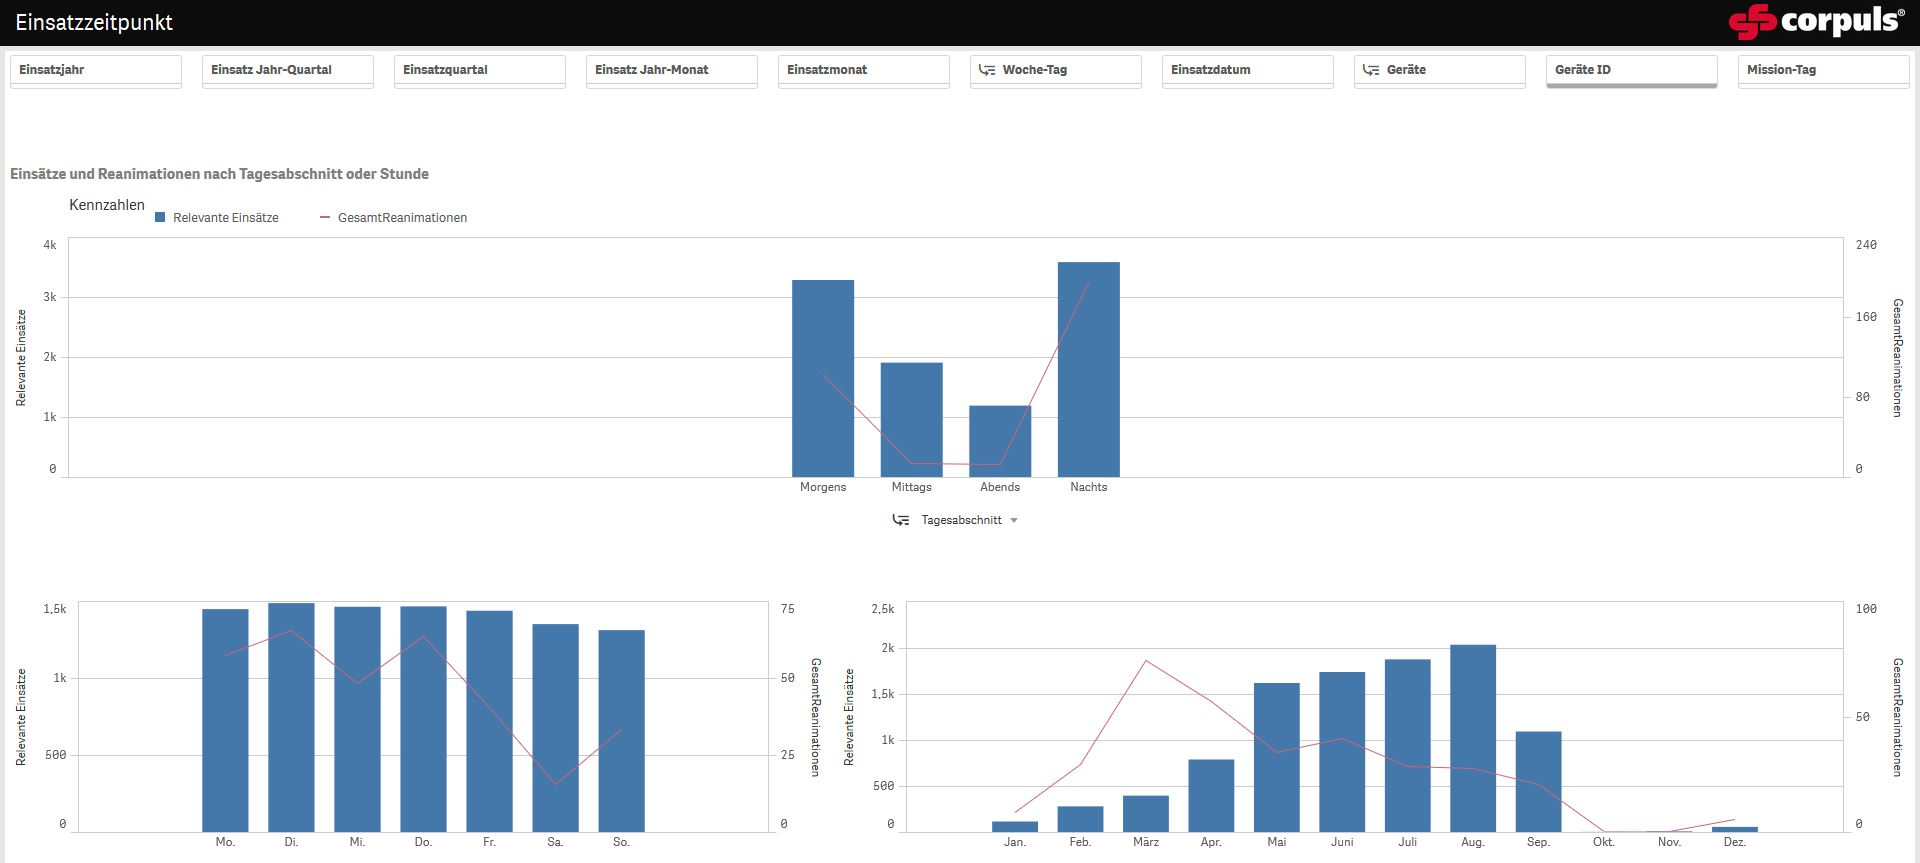
\includegraphics[width=1\linewidth]{img/beforeCT}  
  \caption{Darstellung im Standard-Theme von Qlik Sense}
  \label{fig:beforeCT}
\end{subfigure}
\begin{subfigure}{1\linewidth}
  \centering
  % include second image
  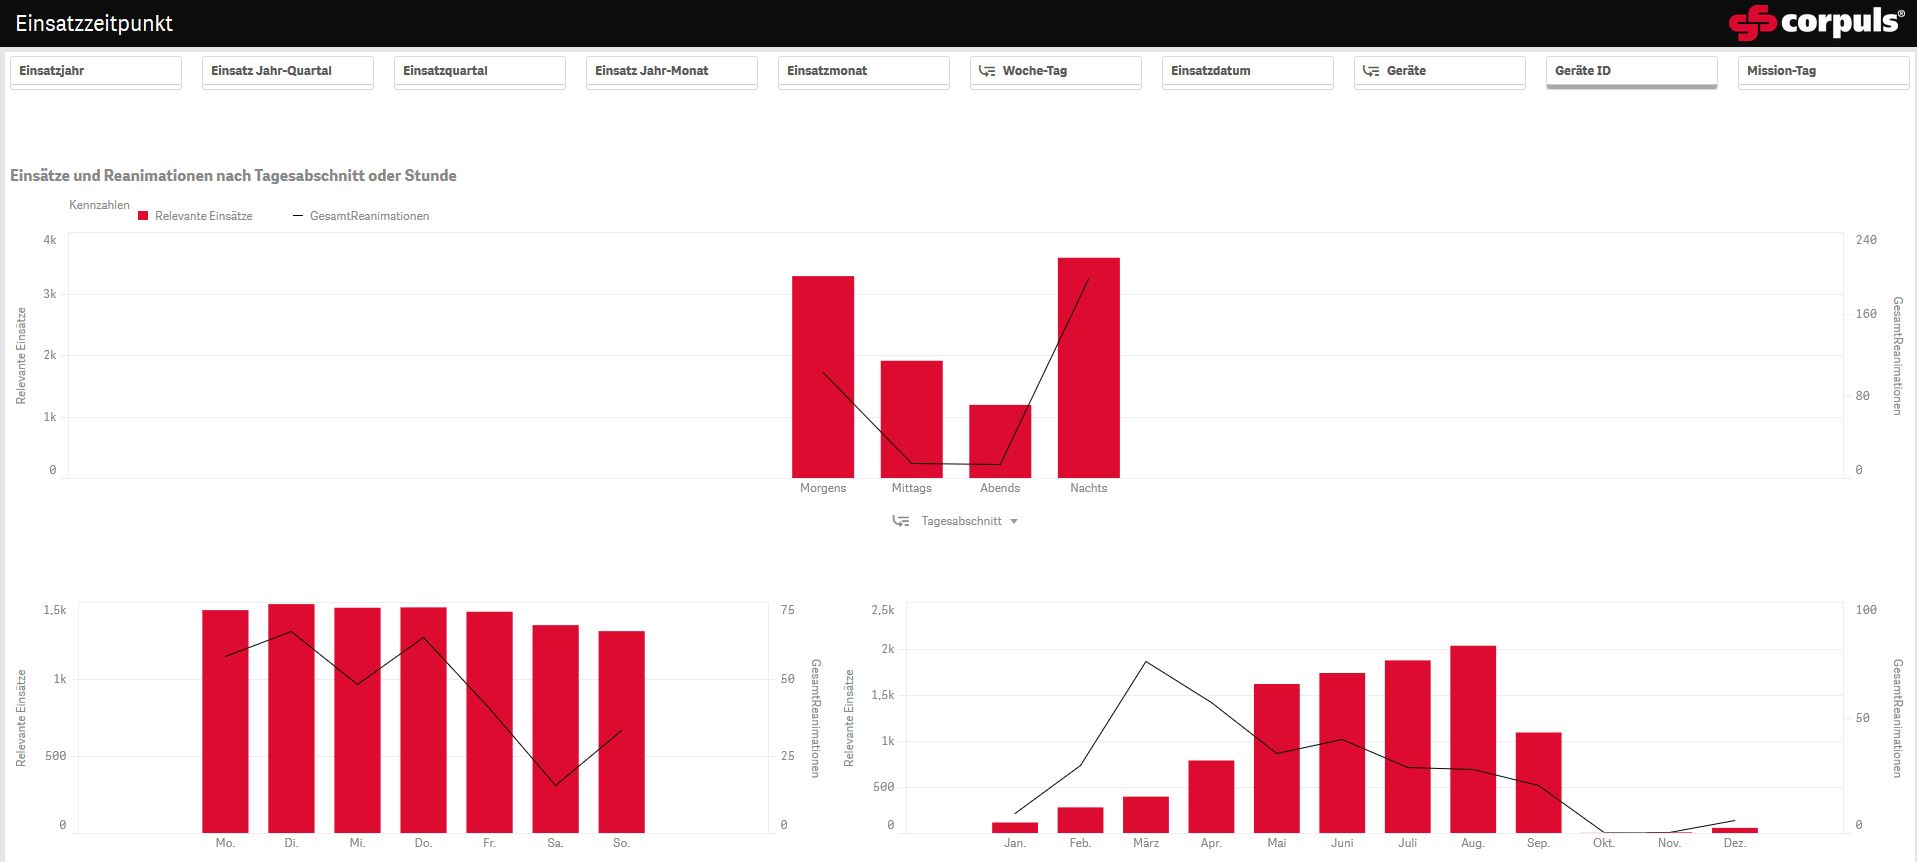
\includegraphics[width=1\linewidth]{img/afterCT}  
  \caption{Umsetzung eines Custom-Themes mit Corporate Design}
  \label{fig:afterCT}
\end{subfigure}
\caption[Vergleich zwischen Standard- und Custom-Theme]{Vergleich zwischen Standard- und Custom-Theme. In }
\label{fig:custom}
\end{figure}

Dementsprechend wurde eine Erweiterung mit den notwendigen Dateien angelegt.
Von Relevanz ist hierbei die JSON-Datei, welche die entsprechenden Werte der Darstellung verändert.
Diese ist im Anhang \todo{\ref{att:json} attach json} zu sehen.

Die Auswirkung der veränderten Farbgebung ist in Abbildung \ref{fig:custom} zu erkennen. 
Es sind in \ref{fig:afterCT} die Farben des Firmen-Logos (zu sehen in der rechten oberen Ecke) auf die Diagramme angewandt worden.
Dadurch herrscht ein Einklang mit der Produktfamilie \textsf{corpuls\color{corpulsred}{.web}} und eine äußere Konsistenz ist gegeben.

%anhang json

%\subsection{Einstellungen der Arbeitsblätter und Diagramme}
% (wie zB. Farben bei Auswahl beibehalten)

%\section{Evaluierung der Ergebnisse?}
%subs Usability-Tests?